
\begin{figure*}[htbp]
\centering
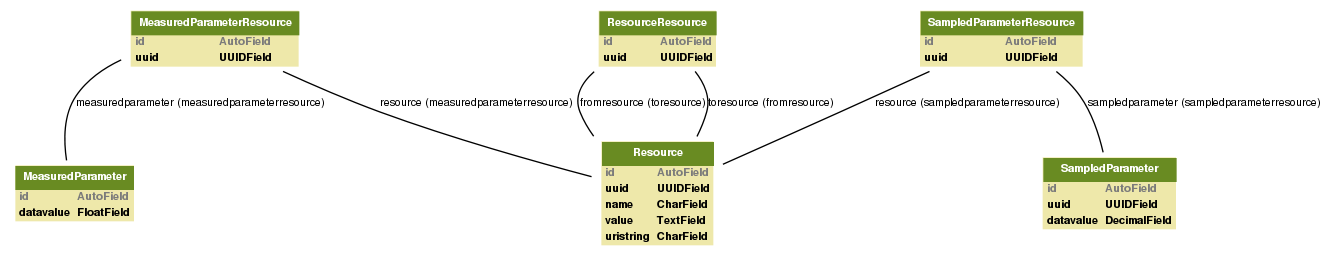
\includegraphics[width=6.6in]{stoqs_simple_model_labels.png}
\caption{Portion of the STOQS data model showing how individual sets of measured or sampled data values can be associated with a Resource name. This enables the labeling of data which is essential for many machine learning operations. A RessourceResource association table allows for unlimited metadata association of the label names.}
\label{fig:stoqs_simple_model_labels}
\end{figure*}

\begin{figure*}[htbp]
\centering
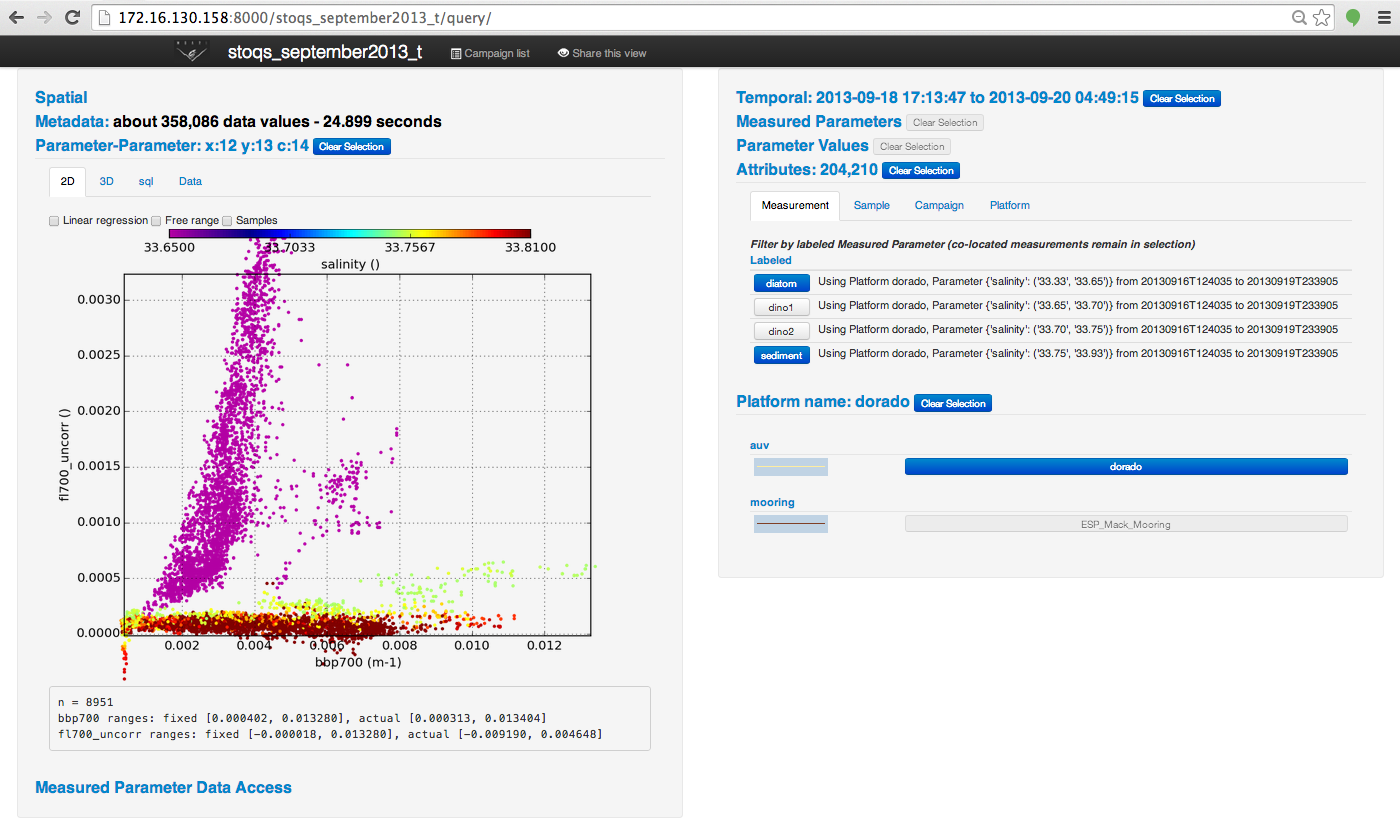
\includegraphics[width=6.6in]{LabeledSelectionUI.png}
\caption{Screen grab of the STOQS UI showing selection of Diatom and Sediment labeled data. The Spatial and Temporal sections of the UI may be explanded to explore the selected data in those dimensions.}
\label{fig:LabeledSelectionUI}
\end{figure*}

\section{Understanding Data}

Today's oceanographic campaigns produce tens of millions of diverse measurements; this volume of data is too great for one to understand all of its information, even with an the effective user interface that STOQS provides.

The same database foundation that enables uniform data access for visualization purposes can be used for analytical purposes. To assist with the operations required by machine learning techniques we have modified the STOQS schema to support labeling of data. This is accomplished by association tables MeasuredParameterResource and SampledParameterReource as shown in Fig.~\ref{fig:stoqs_simple_model_labels}.

By extending the model to support labeled data the other capabilities of STOQS may be used to help understand data. For example, data similar to that shown in Fig.~\ref{fig:JohnsFigureZ} have been labeled with names of Diatom, Dino1, Dino2, and Sediment. These names are exposed through the User Interface as selectable items that may be applied as a filter on the data selection, allowing for easy spatial-temporal exploration of the data within the User Interface.

We are currently exploring ways to enhance data exploration and discovery using both supervised and unsupervised machine-learning methods.  These methods would produce tags that are stored in association tables that can be tied back to the actual data values.  In the future, we envision these tags being further refined through expert validation, or as a feature to other processing, whether it is biological models or further machine learning models. 

The STOQS platform is currently under continued development.  Machine-learning approaches to assess relational patterns within and among multi-platform physical, chemical and biological data already in hand is our current focus.  For example, implementation of additional data labeling within STOQS will empower machine-learning methods to identify and associate specific combinations of optical (e.g., backscatter, transmissometry) or other measurements with biological signals from specific groups of organisms detected in representative water samples (e.g., phytoplankton or zooplankton taxonomic groups). With further development, it may be possible to identify groups of organisms based solely on their specific physical and/or chemical signatures that are more easily measured by in situ electronic sensors.

